\chapter{Microbial Network Modelling}
\pagenumbering{arabic} \setcounter{page}{21}

As stated in the previous chapters, the microbes form associations, which can be studied using the principles of network science. From abundance matrix of sequences to community network models there exist a long chain of essential prcoess. This chapter review the stratgegies involved while making a micorbial cooccurrence networks.

\subsection{Pairwise Interactions}
The associations are primarily classified into three categories,i.e., positive interaction, negative interaction, of neutral interaction. Figure \ref{fig:figure6} shows the graphical summary of the interaction types. The most basic interaction is \emph{mutualism}, which is a win-win scenario for both members of the pair. These members benefit from each other under this association (e.g. co-operative and symbiotic pairs). Opposite to that, the \emph{Competition} association is the lose-lose situation as both the members compete for resources. \emph{Predation} \& \emph{Parasitism} can have win-lose effects on either member as if one is the predator/parasite; the other has to be the prey/host. Following that, in a situation where a member is neutral, and the other member in the pair is being harmed, this kind of association is known as \emph{Amensalism} or \emph{Commensalism} if other benefits. Co-occurrence networks derived using pairwise associations are perceived as simple networks and made using similarity-based inferences as discussed in the previous chapters. Initially, all the normally derived permutation-combinations are used to calculate the mathematical measures and then the significant ones are retained to form co-occurrence networks [Figure \ref{fig:figure7}].

\subsection{Complex Interactions and Dynamic Networks}
The cases may arise when more than one microbial interaction is under study. The associations involve more than two members undergoing either positive, negative or neutral associations. The rules of pair-wise interaction still apply; however, the number of contributing members changes in order to map the complex interactions methods like multiple-regression and associative rule mining is used. The multiple-regression predicts the dependent variable/interaction based on the independent variables/group of pair-wise interactions. The networks so generated are called the directed hypergraphs, which have hyperedges. Figure \ref{fig:figure8} shows a typical complex co-occurrence network made using associative rule mining. The generalized Lotka-Volterra equations used to simulate a dynamic model of a microbial community. As input, they need the growth rates $b_{i}$ and interaction strengths $a_{ij}$ of the different community members, which can either be obtained experimentally or estimated from time-series data. The abundance of taxa $i$ at time $t$ are denoted by $x_{i}(t)$

$$\frac{dx_{i}(t)}{dt} = x_{i}(t)(b_{i} + \sum^{N}_{j=1}a_{ij}x_{j}(t))$$


\begin{figure}
  \centering
  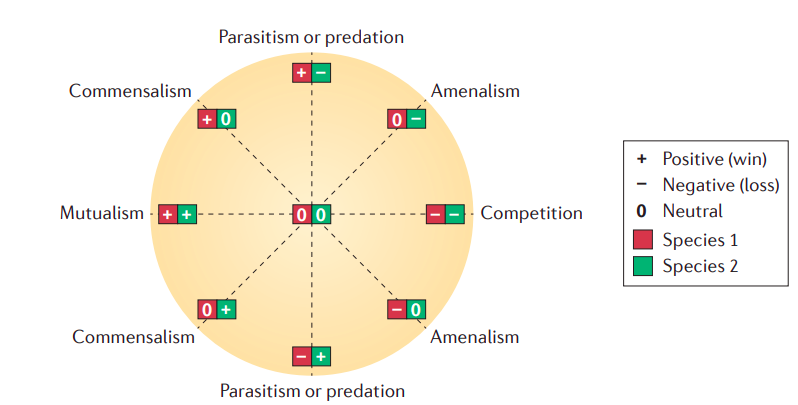
\includegraphics[width=12cm, height=6cm] {../figures/Figure6.png}
  \caption{Typical Rarefaction Curve, It displays how many species are identified with prolonged sampling. If sampling is ample, curves should finally plateau as it becomes tougher to find new species, despite the increase in sampling. On the other hand, if the curves are steep, more sampling is required to infer ecological judgments \cite{ref11}}
  \label{fig:figure6}
\end{figure}

\begin{figure}
  \centering
  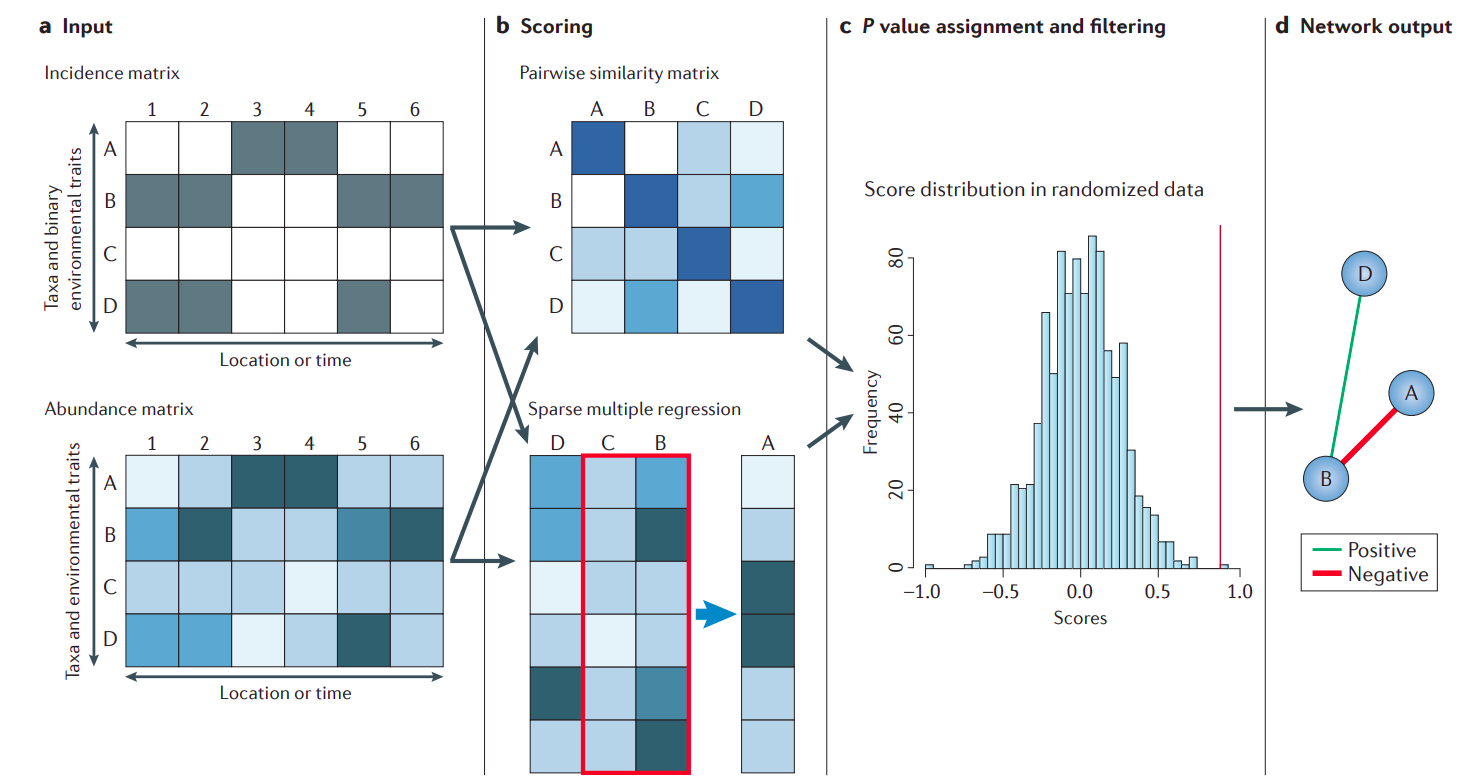
\includegraphics[width=14cm, height=8cm] {../figures/Figure7.png}
  \caption{Typical Rarefaction Curve, It displays how many species are identified with prolonged sampling. If sampling is ample, curves should finally plateau as it becomes tougher to find new species, despite the increase in sampling. On the other hand, if the curves are steep, more sampling is required to infer ecological judgments \cite{ref11}}
  \label{fig:figure7}
\end{figure}

\begin{figure}
  \centering
  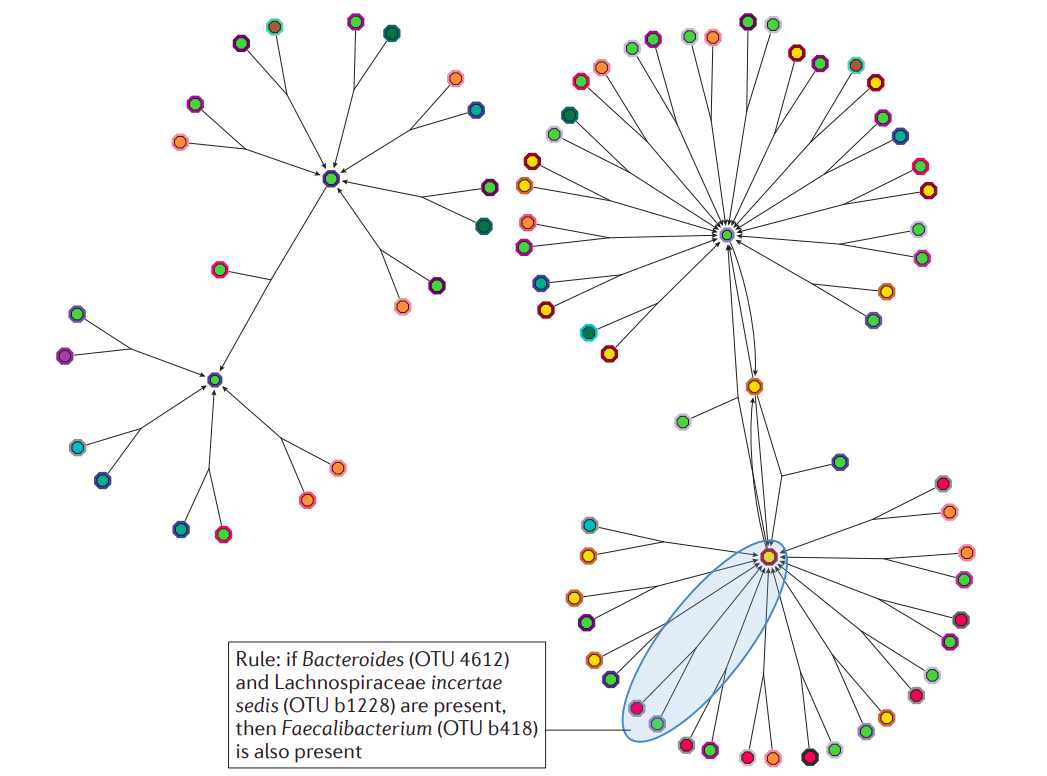
\includegraphics[width=14cm, height=8cm] {../figures/Figure8.png}
  \caption{Typical Rarefaction Curve, It displays how many species are identified with prolonged sampling. If sampling is ample, curves should finally plateau as it becomes tougher to find new species, despite the increase in sampling. On the other hand, if the curves are steep, more sampling is required to infer ecological judgments \cite{ref11}}
  \label{fig:figure8}
\end{figure}
